\edef\mychapter{Rates of Change}
\edef\mychapterdate{July 10, 2024}

\chapter{\mychapter}

\section{Rates of Change}
\subsection{Linear Approximations}
Today, we are going to discuss a pseudo-calculus topic. We are going to try to generalize the idea of a slope onto functions that aren't just straight lines.

As we know from geometry, we can find the equation of a line using only two points. This will become very important since we will use the idea of creating \textbf{linear approximations} of functions. Unfortunately, due to the curvy nature of general functions, we cannot directly apply the idea of the slope, and instead, we have to approximate its slope at a point with a line. Let's see how this works with an example.
\begin{ex}
	In this example, I'd like to find the linear approximation for the function
	$$f(x)=5x^3+2x+3$$
	for the point $(1,f(1))$. 
	We know from previous math classes, that if we had two points, we could generate a line through those points and find its slope. Therefore, we must find two points the point $(1,f(1))$, where we can draw a line through it.
	
	For now, let's use the point $(0,f(0))$ and $(2,f(2))$. To find the line that goes through these points, we use the formula
	$$\frac{f(b)-f(a)}{b-a}=\frac{f(2)-f(0)}{2-0}=\frac{47-3}{2}=22$$
	Then using point-slope form, we get 
	$$y-f(0)=y-3=22x$$
	Hence converting to slope-intercept form, we get the line
	$$y=22x+3.$$
	Then using figure \eqref{fig:averageslope1}, we can see we did a pretty good job here approximating, but I think we can do better.
	
	\begin{figure*}[h]
	\centering
		\resizebox{0.7\textwidth}{!}{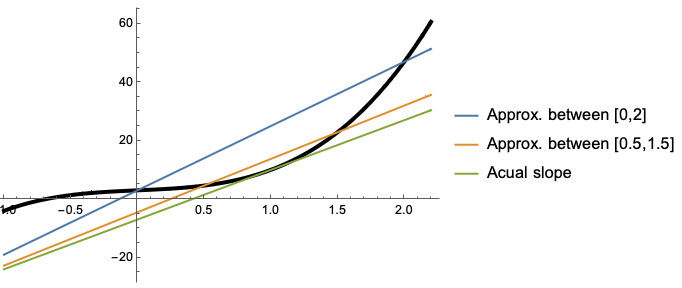
\includegraphics{chapters/assets/RoC/averageslope1.png}}
		\caption{}
		\label{fig:averageslope1}
	\end{figure*}
	
	Let's shrink our interval so we take the line that runs between the points $\paren{\frac{1}{2},f\paren{\frac{1}{2}}}$ and $\paren{\frac{3}{2},f\paren{\frac{3}{2}}}$.
	Using the same formula as before, we get
	$$\frac{f\paren{\frac{3}{2}}-f\paren{\frac{1}{2}}}{1.5-0.5}=\frac{\frac{183}{8}-\frac{37}{8}}{1}=\frac{73}{4}$$
	Therefore our line can be represented as
	$$y=\frac{73 }{4}x-\frac{9}{2}$$
	Then looking back at figure \eqref{fig:averageslope1}, the approximation is way better and a lot closer to what the actual slope is.
\end{ex}

\begin{ex}
	Now let's try a different example. Let's try to make linear approximations for the function
	$$f(x)=x^2-3x+2$$
	for the point $(2,f(2))$. This time, however, instead of taking the interval around this point, let's anchor one point at $x=2$ and set our second point $h$ away from our initial. Writing the general formula for the slope of this line gives
	$$\frac{f(x+h)-f(x)}{h}.\footnotemark$$
	\footnotetext{This is the preferred method for finding linear approximations since very easily, we can take this approximation to 0, which will give us the actual slope of a point on an arbitrary function.}
	First, let's let $h=1$. Then we find the slope is
	$$\frac{f(3)-f(2)}{1}=2$$
	Therefore computing the line through these two points gives
	$$y=2x-4$$
	\begin{figure*}
	\centering
		\resizebox{0.7\textwidth}{!}{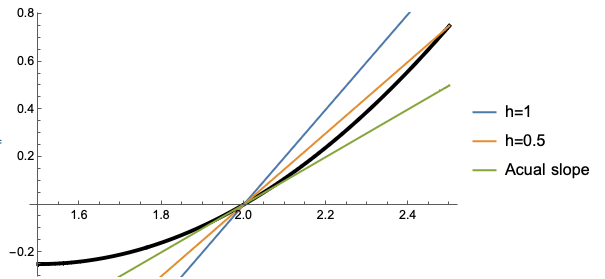
\includegraphics{chapters/assets/RoC/averageslope2.png}}
		\caption{}
		\label{fig:averageslope2}
	\end{figure*}
	Plotting these lines like in figure \eqref{fig:averageslope2}, we see that our approximation is pretty, good, but we do better with smaller and smaller values of $h$. But if we notice, using $h=0$ gives us a divide by zero so finding this value is going to be a bit tricky. Thankfully, we've learned a handy trick for computing values that are masked by dividing by zero errors.
\end{ex}

\subsection{Tangent Line Approximations}
In this section, let's try to take the approximation to 0. As seen in previous examples, as we shrink the interval of the approximation, the line gets closer and closer to its actual approximation, or its \textbf{tangent line} approximation. Let's try to create a tangent line approximation in the following example.

\begin{ex}
	Let's find the tangent line approximation for the function
	$$f(x)=x^2-x$$
	on the point $(1,f(1))$.
	We know the formula for the approximate slope of a point generally is given by
	$$\frac{f(x+h)-f(x)}{h}.$$
	Now let's compute this as $h\to0$ in general in a limit. 
	$$\lim_{h\to0}\frac{f(x+h)-f(x)}{h}=\lim_{h\to0}\frac{((x+h)^2-(x+h))-(x^2-x)}{h}$$
	$$=\lim_{h\to0}\frac{(x^2+2xh+h^2-(x+h))-(x^2-x)}{h}$$
	$$=\lim_{h\to0}\frac{2xh+h^2-h}{h}$$
	Even though $h=0$ causes a divide by zero, as we take the limit to a value, we eliminate that point from our domain, as in the definition of a limit. In this case, we eliminate $h=0$ from our domain, hence dividing out the $h$ here is valid. Therefore
	$$=\lim_{h\to0}2x-h+1$$
	Now since this is a nice smooth function, by plotting it, we can easily tell the limit as $h\to0$ is just whatever the function outputs, hence
	$$=2x+1$$
	This is our tangent line approximation, and if we substitute in $x=1$, we get the slope at this point is 
	$$2(1)-1=1,$$
	hence using the same technique as before, we get the tangent line is
	$$y=x-1$$
	which we can see plotted in figure \eqref{fig:tang1}
	\begin{figure*}
	\centering
		\resizebox{0.6\textwidth}{!}{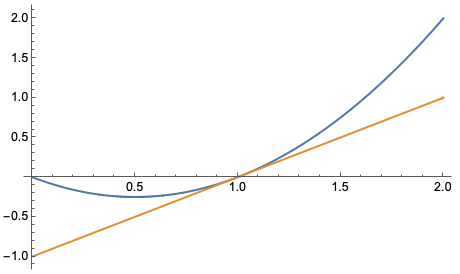
\includegraphics{chapters/assets/RoC/tangent1.png}}
		\caption{}
		\label{fig:tang1}
	\end{figure*}
	\label{ex:tan1}
\end{ex}

Now, let's compute the slope of the tangent line approximation in general. But before doing so, we're going to need some help from the following theorem.

\begin{thm}[Binomial Theorem\footnotemark]
Let $n\in\mathbb{W}$, then
$$(a+b)^n=\sum^n_{k=0}\binom{n}{k}a^ky^{n-k}\footnotemark$$
\label{thm:binomial}
\end{thm}
\addtocounter{footnote}{-1}
\footnotetext{You may have seen this theorem with Pascal's triangle.}
\stepcounter{footnote}
\footnotetext{$\binom{n}{k}$ this means combinations. It's computed by the formula $\frac{n!}{k! (n-k)!}$.}
\begin{proof}
	Postponed indefinitely.
\end{proof}

Now armed with this, let's compute this formula in general.

\begin{ex}
	First, let's compute the formula for a monomial, $ax^n$, where $a\in\real$ and $n\in\mathbb{W}$. Using the limit use used in example \eqref{ex:tan1},
	$$\lim_{h\to0}\frac{f(x+h)-f(x)}{h}=\lim_{h\to0}\frac{a(x+h)^n-ax^n}{h}$$
	Using some theorems we established about limits in Lesson 4, assuming both limits exist,
	$$=\lim_{h\to0}a \cdot \lim_{h\to0}\frac{(x+h)^n-x^n}{h}$$
	Since by plotting $y=a$ we know
	$$\lim_{h\to0}a=a$$
	the only remaining question is if the right-hand limit exists. But can confirm that by continuing our computation.
	Then expanding the binomial with theorem \eqref{thm:binomial}, we get
	$$a  \lim_{h\to0}\frac{(x+h)^n-x^n}{h}
	=a \lim_{h\to0}\frac{\sum^n_{k=0}\binom{n}{k}x^kh^{n-k}-x^n}{h}$$
	$$=a \lim_{h\to0}\frac{\sum^{n-1}_{k=0}\binom{n}{k}x^kh^{n-k}}{h}$$
	Then since here, everything is a factor of $h$ and we can eliminate $h=0$ from our domain, dividing out $h$ gives
	$$=a \lim_{h\to0}\paren{\sum^{n-1}_{k=0}\binom{n}{k}x^kh^{n-k-1}}$$
	Then using the same idea as in example \eqref{ex:tan1}, we can substitute $h=0$, therefore every term that is a factor of $h$ vanishes in our sum. Therefore for $n>0$,
	$$=a \binom{n}{n-1}x^{n-1}$$
	Since
	$$\binom{n}{n-1}=\frac{n!}{{(n-1)}!(1!)}=n$$
	Therefore the general formula for the slope of a tangent line approximation is
	$$anx^{n-1}.$$
	Then for $n=0$, since we start our summation at $0$, nothing is output by the sum, hence our rate of change is 0. \footnote{This is called the power rule in calculus. We can generalize this to all rational exponents if we expand our binomial theorem to become the binomial series.}
	\label{ex:gentan}
\end{ex}

In example \eqref{ex:gentan}, we only computed the slope if the polynomial was one term. To generalize to all polynomials, we need to know how these slopes add. 

\begin{thm}
	Suppose $f,g$ are both polynomials. If $f',g'$ are functions that produce the slope of their tangent line approximations, then the slope of the tangent line approximation of their sum is given as
	$$(f+g)'=f'+g'.$$
	\label{thm:dersum}
\end{thm}
\begin{proof}
	Computing $(f+g)'$ gives
	$$(f+g)'=\lim_{h\to0}\frac{(f+g)(x+h)-(f+g)(x)}{h}$$
	$$=\lim_{h\to0}\frac{(f(x+h)-f(x))+(g(x+h)-g(x))}{h}$$
	Then by limits laws, we know
	$$=\lim_{h\to0}\frac{f(x+h)-f(x)}{h}+\lim_{h\to0}\frac{g(x+h)-g(x)}{h}.$$
	Of course, to make this conclusion, we need to know these limits exist, but since we know
	$$f'(x)=\frac{f(x+h)-f(x)}{h} \jand
		g'(x)=\frac{g(x+h)-g(x)}{h}$$
	this is the case, therefore
	$$=f'+g'$$
\end{proof}

Now with theorem \eqref{thm:dersum}, we can compute the slope of the tangent line with any arbitrary polynomial. Let's try this with the following example.

\begin{ex}
	Let's compute a general formula for the tangent line for the polynomial
	$$P(x)=x^5+2x^2+x-5$$
	Using the formula we computed in example \eqref{ex:gentan}, we can compute the slope of the tangent line for each monomial. Doing so gives us
	$$(x^5)'=5x^4$$
	$$(2x^2)=4x$$
	$$(x^1)'=1$$
	$$(-5x^0)'=0$$
	Then using theorem \eqref{thm:dersum},
	$$P'(x)=5x^4+4x+1$$
	Therefore, for any point $(x,P(x))$, the tangent line in point-slope form is
	$$y-P(x)=P'(x)(w-x)$$
	\begin{figure*}[h]
		\centering
		\resizebox{0.6\textwidth}{!}{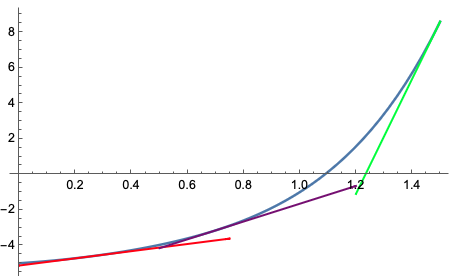
\includegraphics{chapters/assets/RoC/tanplot1.png}}
		\caption{}
		\label{fig:tanplot1}
	\end{figure*}
	where $w$ is the independent variable. In figure \eqref{fig:tanplot1}, you can see a couple of them plotted.
\end{ex}

\section{Plotting Polynomials}
\subsection{Local Extrema}
\begin{define}
	Define $f:\mathcal{D}\to\real$, where $\mathcal{D}\subseteq\real$. If there exists an open interval $(a,b)\subseteq\mathcal{D}$ such that $c\in(a,b)$, is the maximum value, then $c$ is a \textbf{local maximum}.
\end{define}
\begin{define}
	Define $f:\mathcal{D}\to\real$, where $\mathcal{D}\subseteq\real$. If there exists an open interval $(a,b)\subseteq\mathcal{D}$ such that $c\in(a,b)$, is the minimum value, then $c$ is a \textbf{local minimum}.
\end{define}

The mathematical jargon might be difficult to navigate, but all the two definitions is saying is that if a point on a function function is a maximum on an interval, where this point is not on the boundary, then this point is a local maximum. Or as in figure \eqref{fig:localmax}
\begin{figure*}[h]
	\centering
	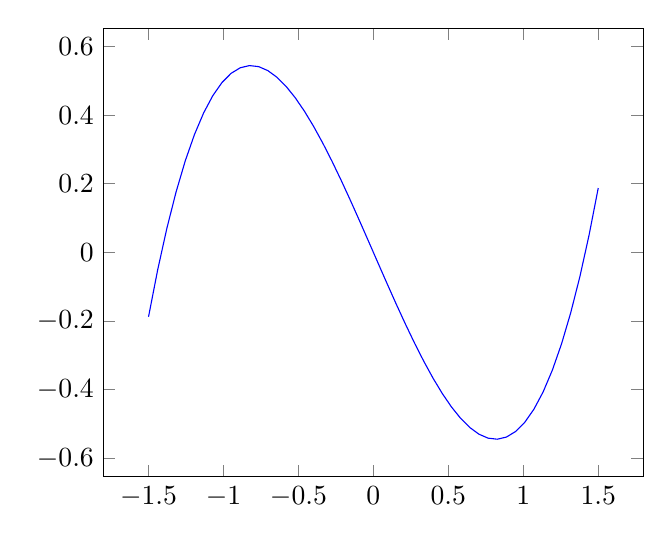
\begin{tikzpicture}
		\begin{axis}
			\addplot[blue, domain=-1.5:1.5,samples=50] {1/2*x^3-x};
			
		\end{axis}
	\end{tikzpicture}
	\caption{}
	\label{fig:localmax}
\end{figure*}









